\documentclass{article}
\usepackage{graphicx} % Required for inserting images
\usepackage{hyperref}

\title{Project 2: Rush Hour}
\author{4 guys}
\date{May 2024}

\begin{document}

\maketitle

\section{The Premise}
Rush Hour is a solitaire game where the player moves cars and trucks forward and backward on a 6x6 grid to try and free a red car that is trying to leave. All cars have dimensions 2x1 and all trucks have dimensions 3x1. The difficulty lies in the fact that none of the cars can turn and that the grid is relatively small and filled with obstructive vehicles.

\begin{figure}
    \centering
    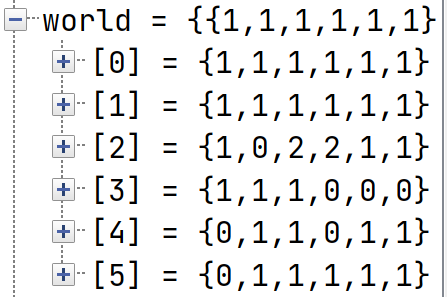
\includegraphics[width=0.5\linewidth]{images/movematrix.png}
    \caption{The world matrix, initialized on the hardest configuration}
\end{figure}

\section{Our Model}
\subsection{The Grid}
The grid is modelled using a 6x6 matrix, called the world matrix. 0s on this matrix indicate no vehicle is in that location, 1s indicate a car or truck, and 2s indicate the red car. By having the processes that model our cars avoid entering tiles that are not 0s we avoid collisions and guarantee that the cars behave as they should.

\begin{figure}
    \centering
    
\includegraphics[width=1\linewidth]{images/params.png}
    \caption{The car parameters}
\end{figure}

\subsection{The Vehicles}
Every vehicle in our model is modeled as its own process, all the cars share a template, and all the trucks share a template. We can conveniently determine if a vehicle can move vertically or horizontally, and determine its starting position on the grid by varying its parameters. The first parameter determines which direction the car is facing, with 0 indicating horizontal movement, and 1 indicating vertical movement. The next two parameters indicate the x and y positions of the front of the car. The red car has its own template because it only ever faces horizontally\footnote{Updating the red car process to accommodate vertical movement would be relatively simple}, so it doesn't need the edges for vertical movement. Additionally, it needs an extra edge and location that guarantees that it goes to the exit as soon as the opportunity presents itself. This is especially important because that is our winning state.

\begin{figure}
    \centering
    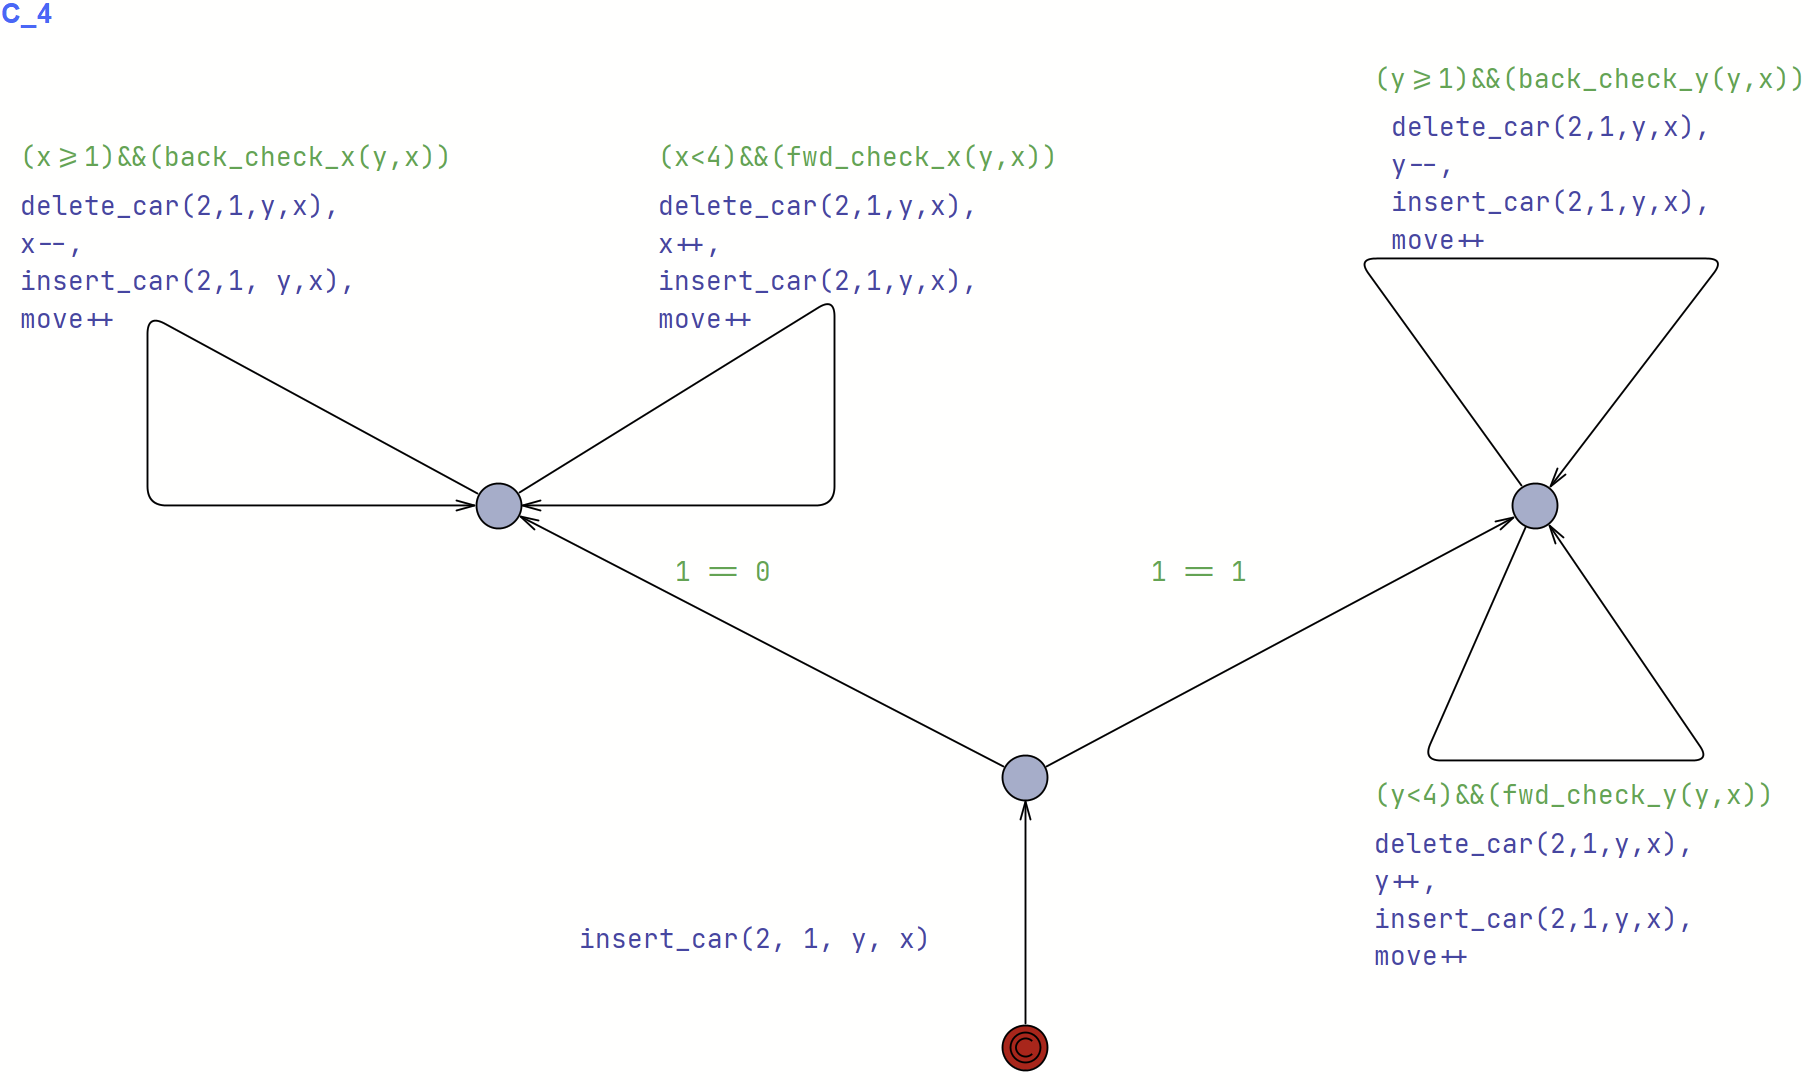
\includegraphics[width=0.9\linewidth]{images/c4.png}
    \caption{The car process}
\end{figure}

\begin{figure}[hbt!]
    \centering
    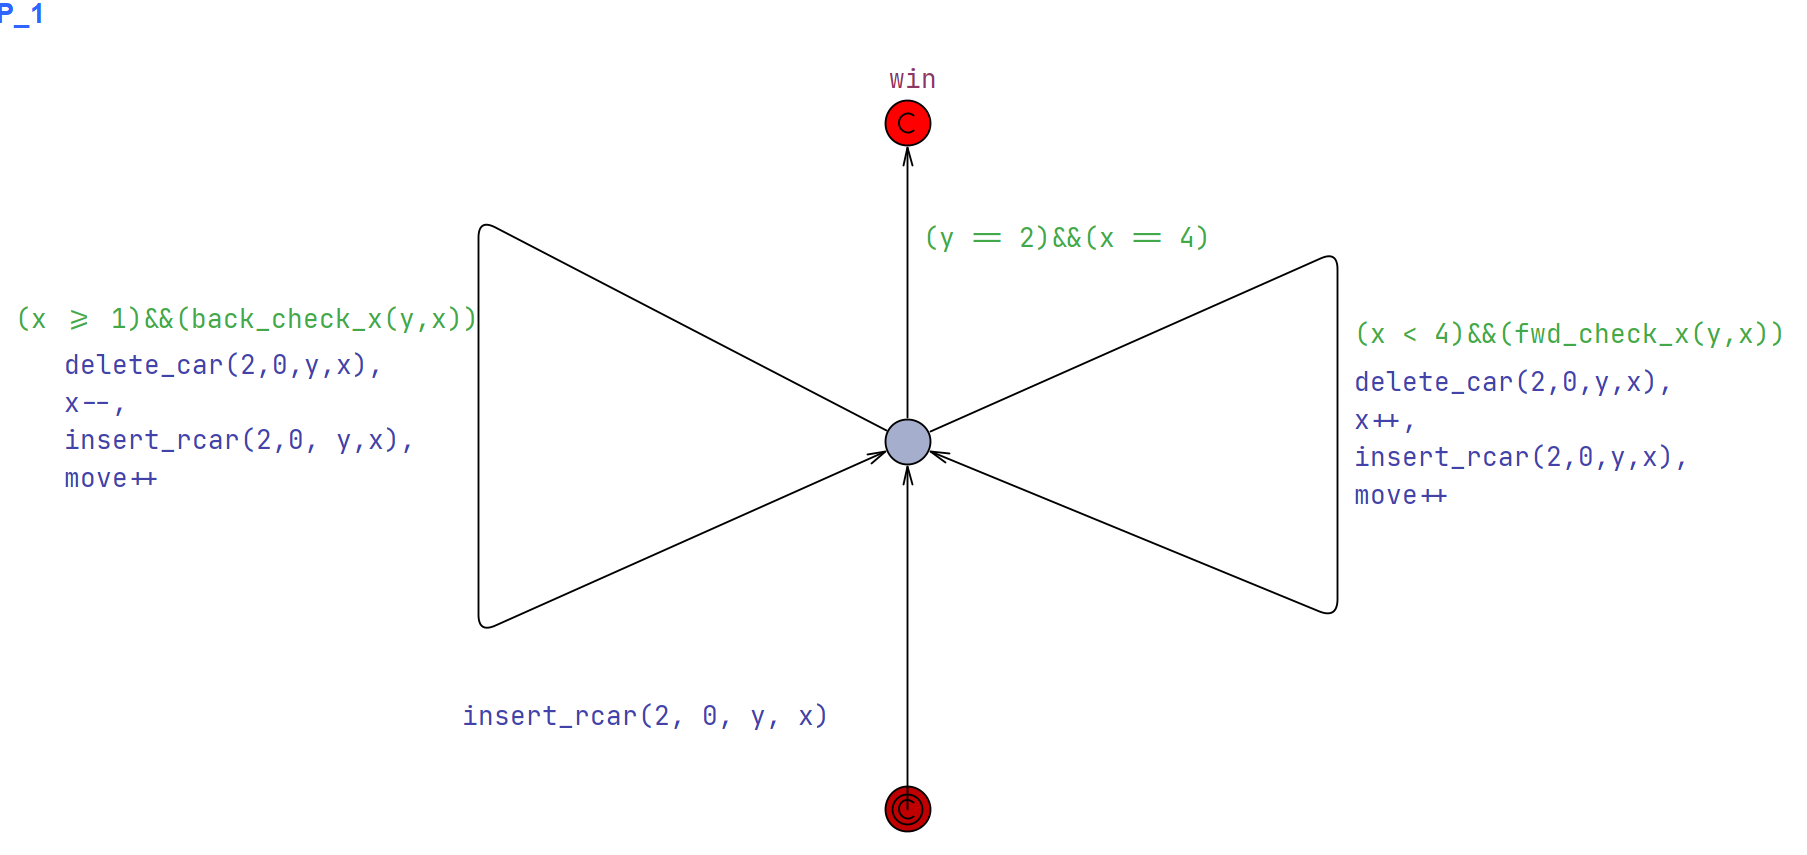
\includegraphics[width=0.8\linewidth]{images/redcar.png}
    \caption{The red car process}
\end{figure}

\begin{figure}[hbt!]
    \centering
    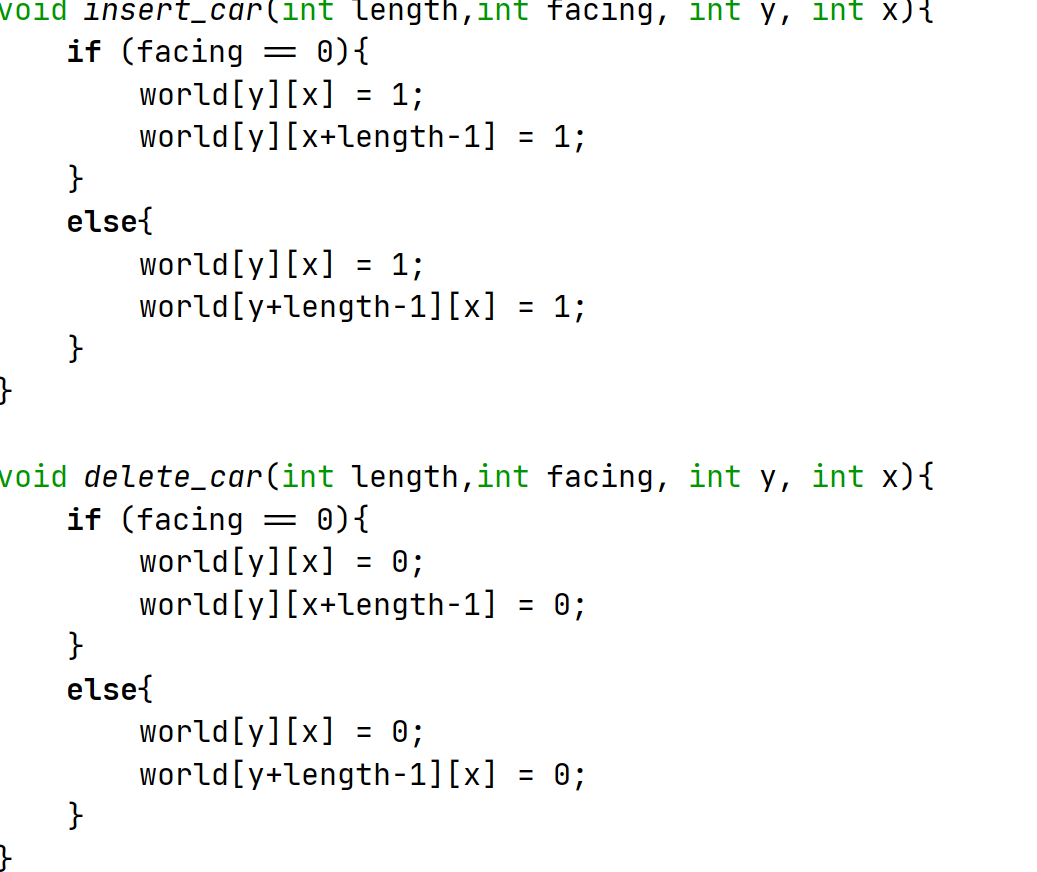
\includegraphics[width=0.75\linewidth]{images/insertdelete.png}
    \caption{The insert\_car, and delete\_car functions}
\end{figure}

\subsubsection{Initializing The Matrix}
We use the \emph{insert\_car} function to insert our cars into the matrix. It checks if the car is facing vertically or horizontally and then fills in the appropriate entries of the matrix with 1s. The red car uses the \emph{insert\_rcar} function that fills in the matrix with 2s rather than 1s, and trucks use the \emph{insert\_truck} function, which has an added line of code that adds the third portion of the truck. To guarantee that all the vehicles run through these functions before UPPAAL tries to solve the game all the vehicle processes begin on a committed location to force them to move through the edge that runs these functions.

\begin{figure}[hbt!]
    \centering
    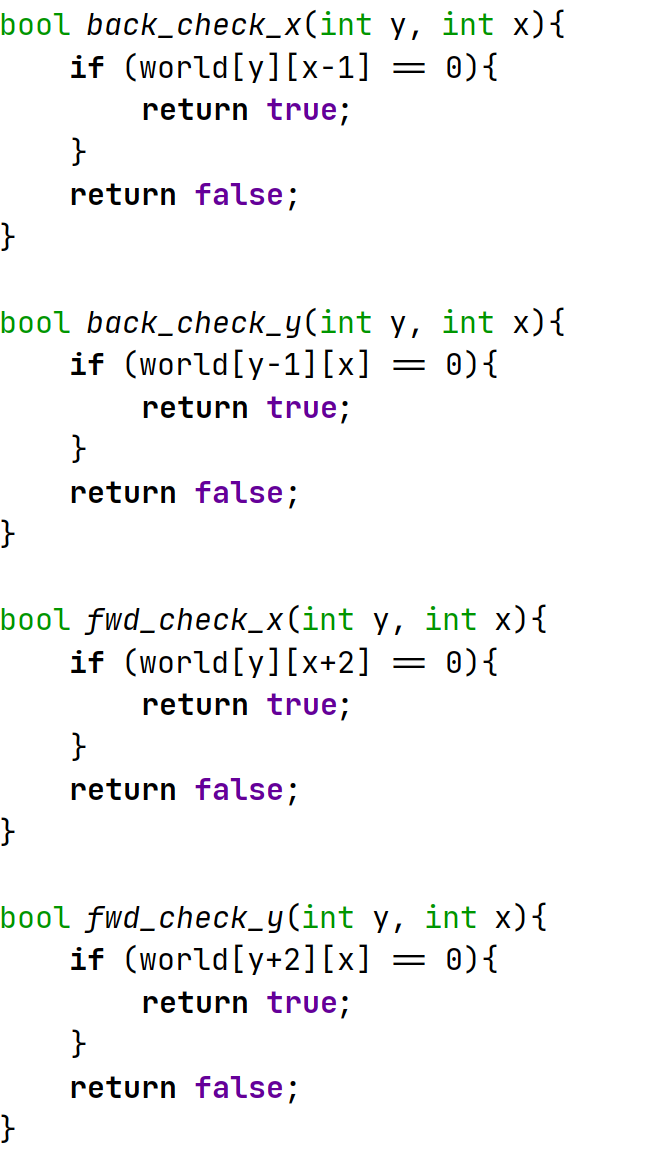
\includegraphics[width=0.5\linewidth]{images/checks.png}
    \caption{The check functions}
\end{figure}

\subsubsection{Guards and Edges}
Once the vehicles have all moved through the edges that initialize the matrix they can move to the most used portion of their processes. In non-red vehicles the process branches off into two sections, the guards on these branches guarantee that the vehicles go to the section that corresponds to the movement indicated by their faces. Once the vehicles reach the appropriate section each traversal of an edge corresponds to that vehicle moving 1 tile. These edges have guards that prevent them from leaving the grid, and guard functions that check to make sure the tiles they move into only contain 0s, as moving into any tile not containing a 0 would cause a collision. The update code on these edges moves the vehicles.

\subsubsection{Moving}
The vehicles in our model don't exactly move, they are repeatedly deleted from where they are, and then inserted where they're supposed to end up after moving one tile. This solution is elegant because it reuses the functions for initializing the matrix. The delete functions work relatively similarly to the insert functions, in that they check which direction the vehicle is facing and then turn the appropriate entries of the matrix into 0s. There is no \emph{delete\_rcar} function because the absence of a red car is the same as the absence of any other car in our model, they're all represented by 0s, so the \emph{delete\_car} function is sufficient.

\section{The Query}
$\exists \diamond P\_1.win$ This is our query for all versions of the problem. It simply asks UPPAAL to find a set of actions that allow the red car process (denoted as P\_1) to enter its winning location, which is only accessible if the red car has already moved to the exit tile.


\section{Problems}
Solutions to configurations that we solved with the constraints of all of these problems can be found in our UPPAAL files, they are set up to initialize themselves, and running the query through the verifier will give the correct solution.

\subsection{Problem 3}
Problem 3 is the simplest version of the rush hour problem, our model has to traverse some relatively easy configurations of the grid.
\begin{itemize}
    \item Puzzle card 13 is 32 moves.
    \item Puzzle card 21 is 49 moves.
\end{itemize}

\begin{figure}[hbt!]
    \centering
    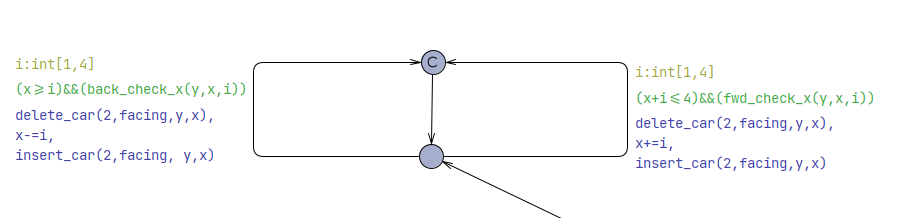
\includegraphics[width=1\linewidth]{images/bonus1template.png}
    \caption{The car process for bonus problem 1}
\end{figure}
\newpage
\subsubsection{Bonus Problem 1}
The premise of this problem is that one step in our model should allow any vehicle to move any number of tiles, as long as moving to that location would be a legal move. \newline
 The overall architecture (e.g. the number of edges) remained the same, however, our functions did need to be modified. We implemented the \emph{back\_check} and \emph{front\_check} functions with for loops (we discovered some limitations of the Uppaal compiler which made this part a bit trickier) so that it was able to check for all of the tiles for the desired move. We added \emph{select} onto our move edges so Uppaal could decide on the number of moves, and edited our guards accordingly so that the vehicle couldn't go out of bounds.
 \begin{figure}
     \centering
     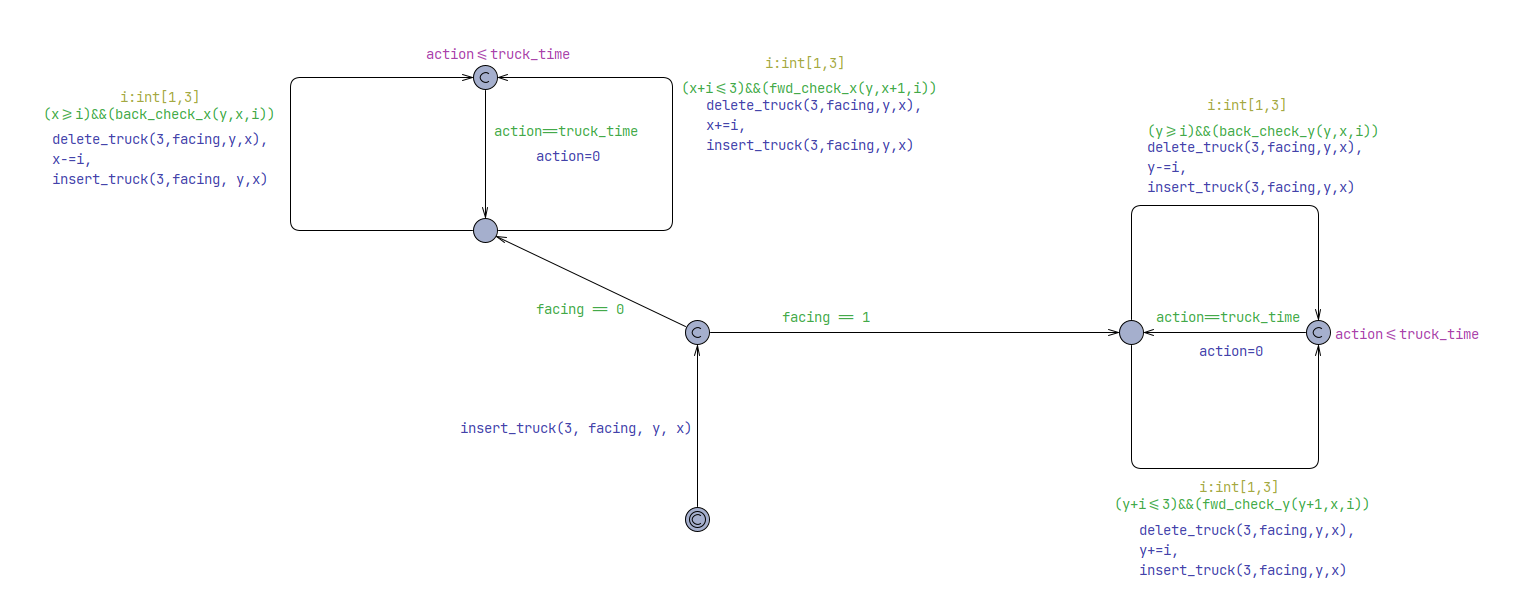
\includegraphics[width=1\linewidth]{images/truck_multimove.png}
     \caption{Truck process}
     \label{fig:enter-label}
 \end{figure}

\subsection{Problem 4}
Problem 4 is seemingly identical to problem 3, however as the configurations are more complex our model struggled a little bit and we had to remove the move counter and replace it with a clock to reduce the state space. 

\newpage
\begin{figure}[hbt!]
    \centering
    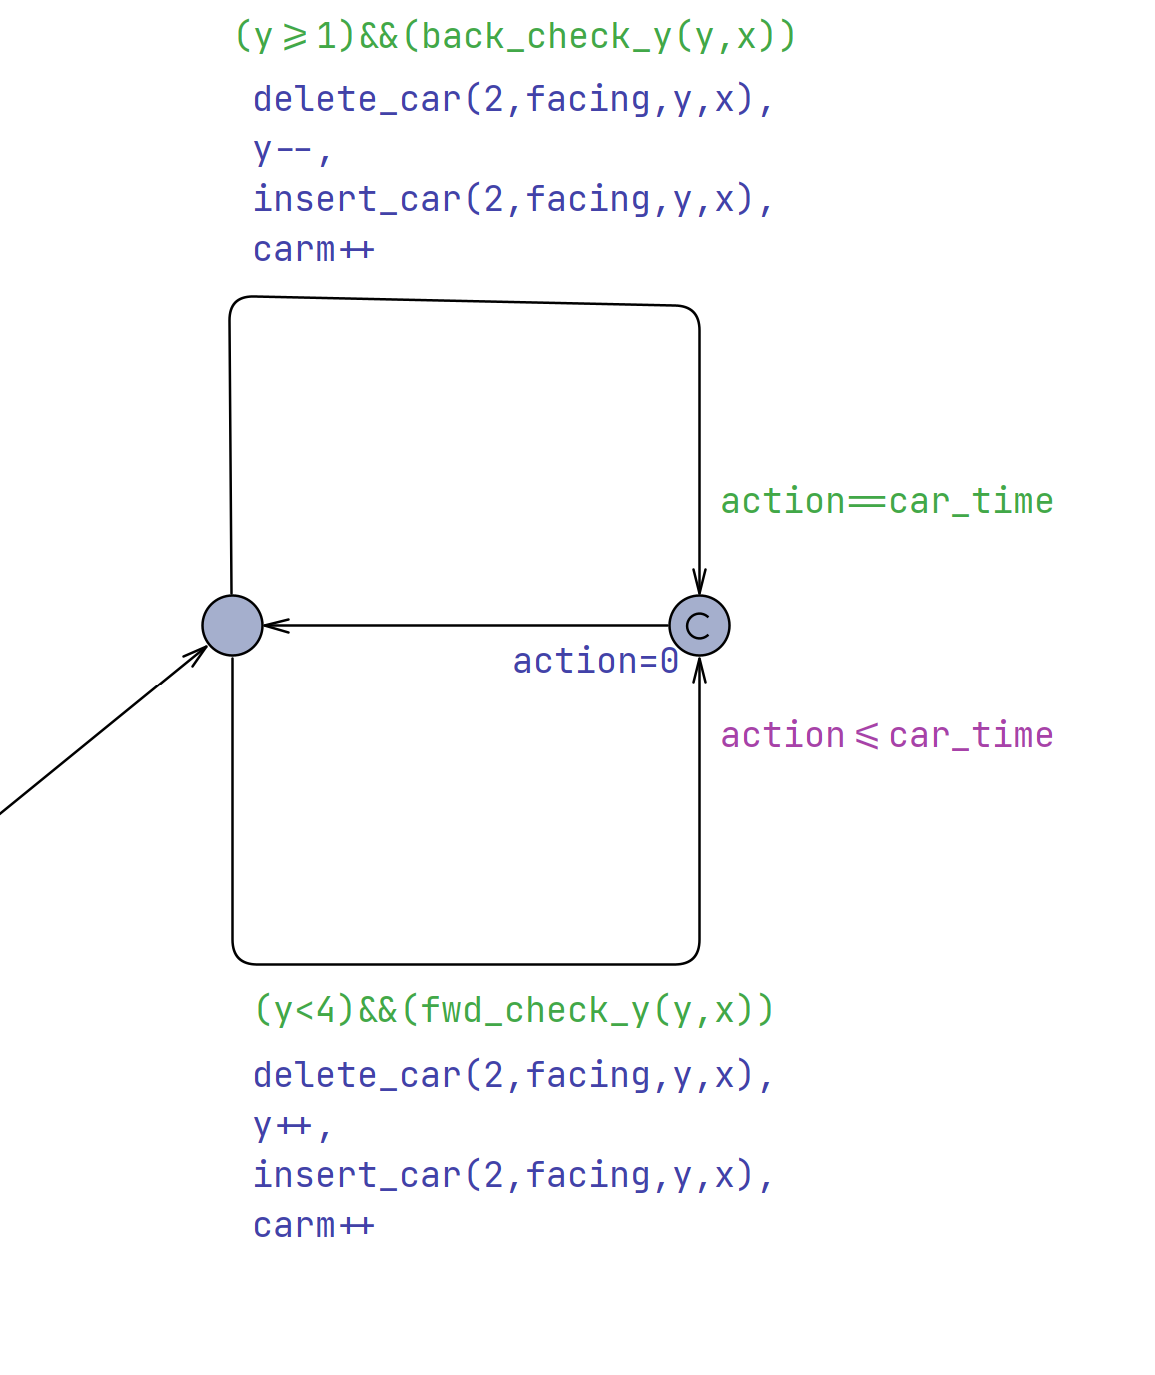
\includegraphics[width=0.75\linewidth]{images/timefix.png}
    \caption{The car process for problem 5 with the extra committed location}
\end{figure}


\subsection{Problem 5}
The premise of this problem is that it takes 2 seconds to move a car and 5 seconds to move a truck.
Modelling this requires adding another committed location to all the movement edges, so that after a vehicle moves, it waits at that committed location the appropriate amount of time, and while it waits the entire model stops, and then the edge back resets the clock. This guarantees that the appropriate amount of time is left between all moves.

\begin{figure}
    \centering
    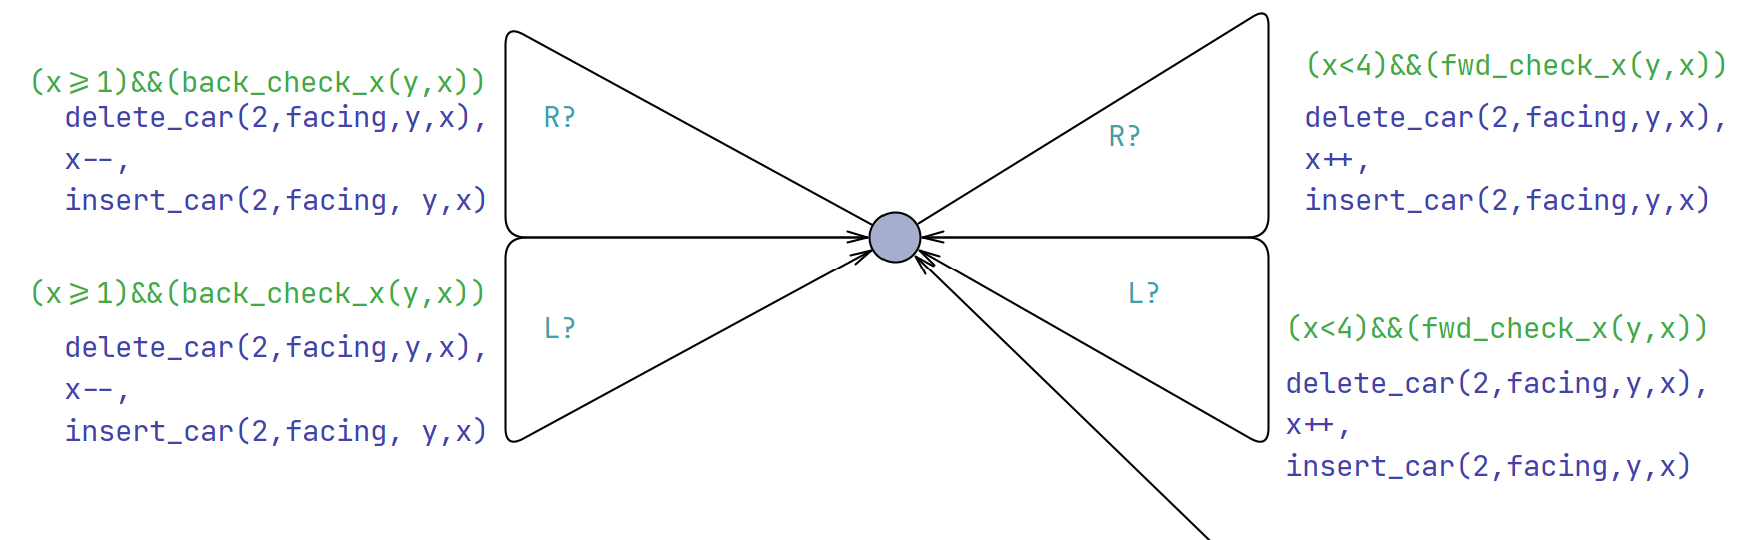
\includegraphics[width=0.9\linewidth]{images/butterfly.png}
    \caption{The car process with duplicated movement edges}
\end{figure}
\begin{figure}
    \centering
    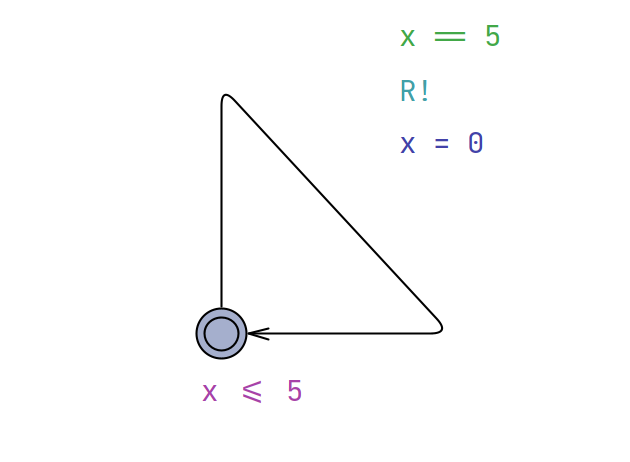
\includegraphics[width=0.5\linewidth]{images/righty.png}
    \caption{The right-hand process, with synchronisation R!}
\end{figure}

\subsubsection{Super Bonus Problem}
The premise of this problem is that you can move vehicles with both hands, but you're left-handed so your left hand takes 3 seconds to move a vehicle, while your right hand takes 5 seconds to move a vehicle.
We modelled this by having each hand be its own process with synchronisation for R! and L! respectively. Then each edge that moves a vehicle needs an R or an L to be traversed. As UPPAAL does not allow two synchronisations to be on the same edge this required duplicating every movement edge in every process in the model. Modelling it this way means that one vehicle could vacate a tile at the same time as another vehicle enters it, which would not be physically possible while sliding objects around on a board. This means solutions generated by this model may not be usable in the real world, or may be a few seconds slower in the real world.\footnote{Avoiding this degree of freedom would require each vehicle to occupy the tile it's leaving, as well as the tile it's moving into for the entire duration of its movement. This would require altering the vehicle processes, and the functions that move vehicles considerably.}

Using this model we solved Rush Hour's hardest configuration 1.1, it took a minimum of 175 seconds, and 93 moves in total. Using this version of the model to solve other configurations would require minimal setup.

\begin{figure}[hbt!]
    \centering
    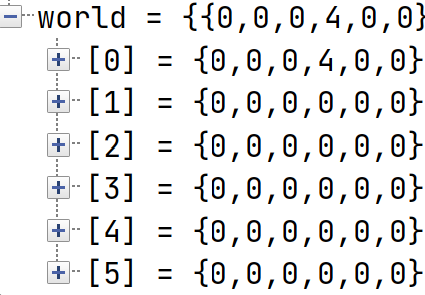
\includegraphics[width=0.5\linewidth]{images/walls.png}
    \caption{The grid with a wall in the position for the first wall problem}
\end{figure}

\subsection{Problem 6}
The premise of this problem is that there are walls on the grid, these walls take up space exactly like a car except they're 1x1 in dimension and cannot move.
Modelling these walls is easy in our model, we simply add a 4 into the grid matrix wherever we want a wall to be, and then let UPPAAL take care of the rest.


\newpage
\subsection{Problem 7 - Quality}
Checking the quality of the model in regards to the criteria discussed by Frits Vaandrager in the article \href{https://www.cs.ru.nl/F.Vaandrager/PV/what_is_a_good_model.html}{What is a Good Model}.
\begin{itemize}
    \item The models have a clearly specified \textbf{object of modelling} and are truthful. The rush hour game can be represented one-to-one by a two-dimensional matrix. In our model the empty spaces are represented by 0s, the red car is represented by 2s and all other cars are represented by 1s. When tackling the more difficult problems time is represented by UPPAALs time module and different hands were represented with their own processes.
    \item The models have a clearly specified \textbf{purpose}, which is to find the best ways to win different rush hour configurations within the boundaries set forth in the problem description.
    \item Our models are somewhat traceable, we traded simplicity for \textbf{traceability} when we made all non-red cars be represented by 1. It could be possible to represent different cars with characters or different numbers but we judged that the added layer of complexity was not worth it. They were however traceable enough that we noticed our cars jumping over other cars on our iteration of the multiple-movement problem.
    \item The models are \textbf{simple} which helps them be \textbf{extensible and reusable}. Re-usability was tested and proven when we could, quite quickly, switch between different setups and solving the hardest problems was only a matter of plugging in the correct starting coordinates. The extensibility of the base models was also tested and proven when problems such as time and two hands were tackled.
    \item The simplicity of the model facilitates \textbf{interoperability and sharing} but we did not specifically design around it and we did not collaborate with other groups in order to determine how easy interoperability would be.
\end{itemize}

\subsection{Final Thoughts}
We quite enjoyed using UPPAAL to model for the assignments and by the end of the course had gained some proficiency in using it to model problems. The rush hour assignment was somewhat more challenging to draw out on a whiteboard compared to Wooldridges vacuum robot which led to us placing greater emphasis on checking the quality of the model instead of drawing out solutions and working out improvements to the model that way. We did run into some problems with syntax constantly and there were a few times where we sorely needed a debugging tool to more easily see what was going wrong.
\end{document}
\begin{figure}
    \centering
    \includegraphics[width=0.5\linewidth]{image.png}
    \caption{The car process}
\end{figure}


